\section{Design}
\label{sec:design}

\begin{figure*}[!bth]
\begin{subfigure}[h]{0.5\textwidth}
\centering
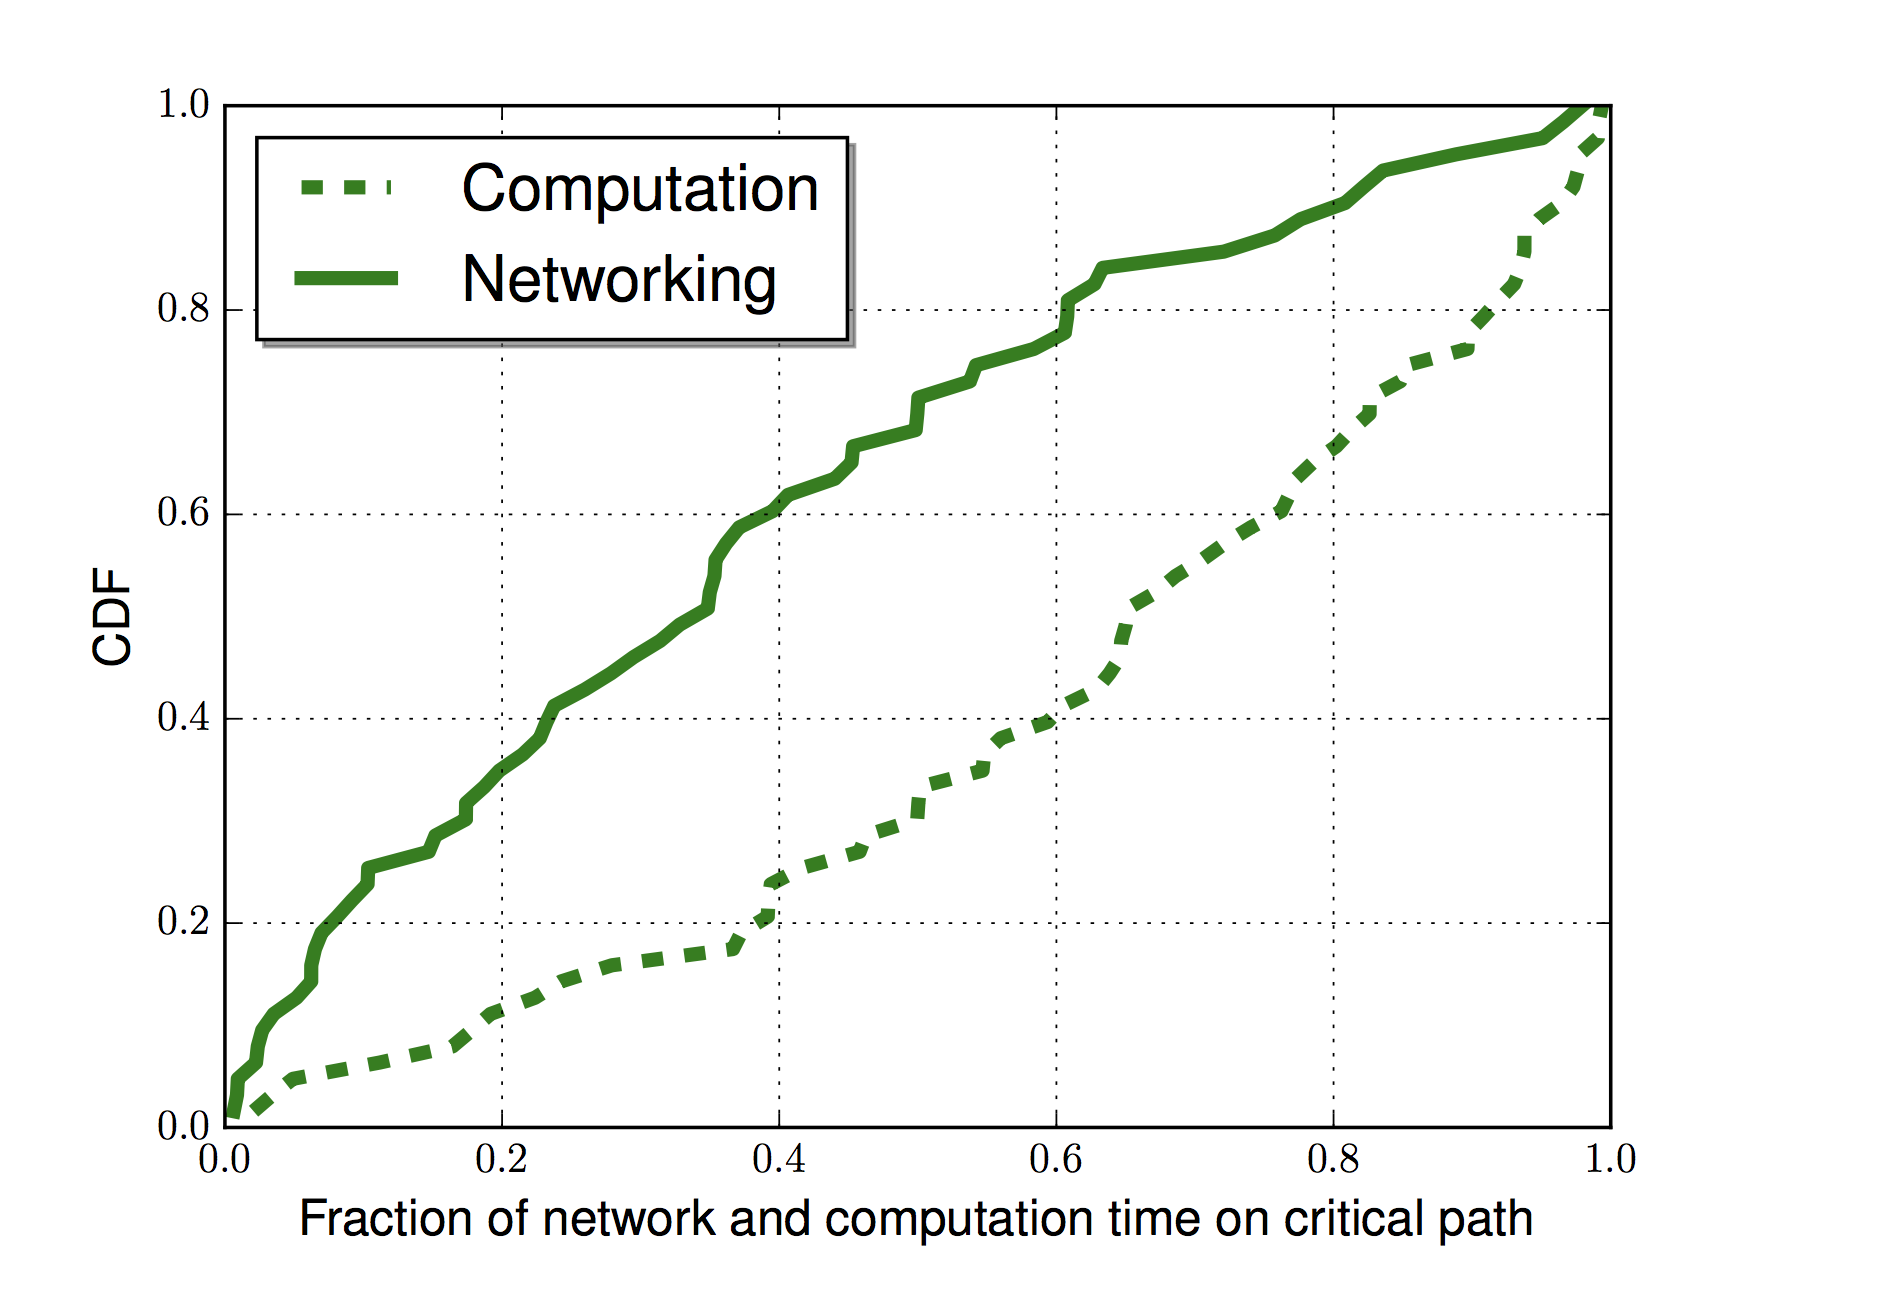
\includegraphics[width=\linewidth]{figs/comp_net.png}
\caption{Runtime information on mobile devices}
\label{fig:mobile-runtime}
\end{subfigure}
\begin{subfigure}[h]{0.5\textwidth}
\centering
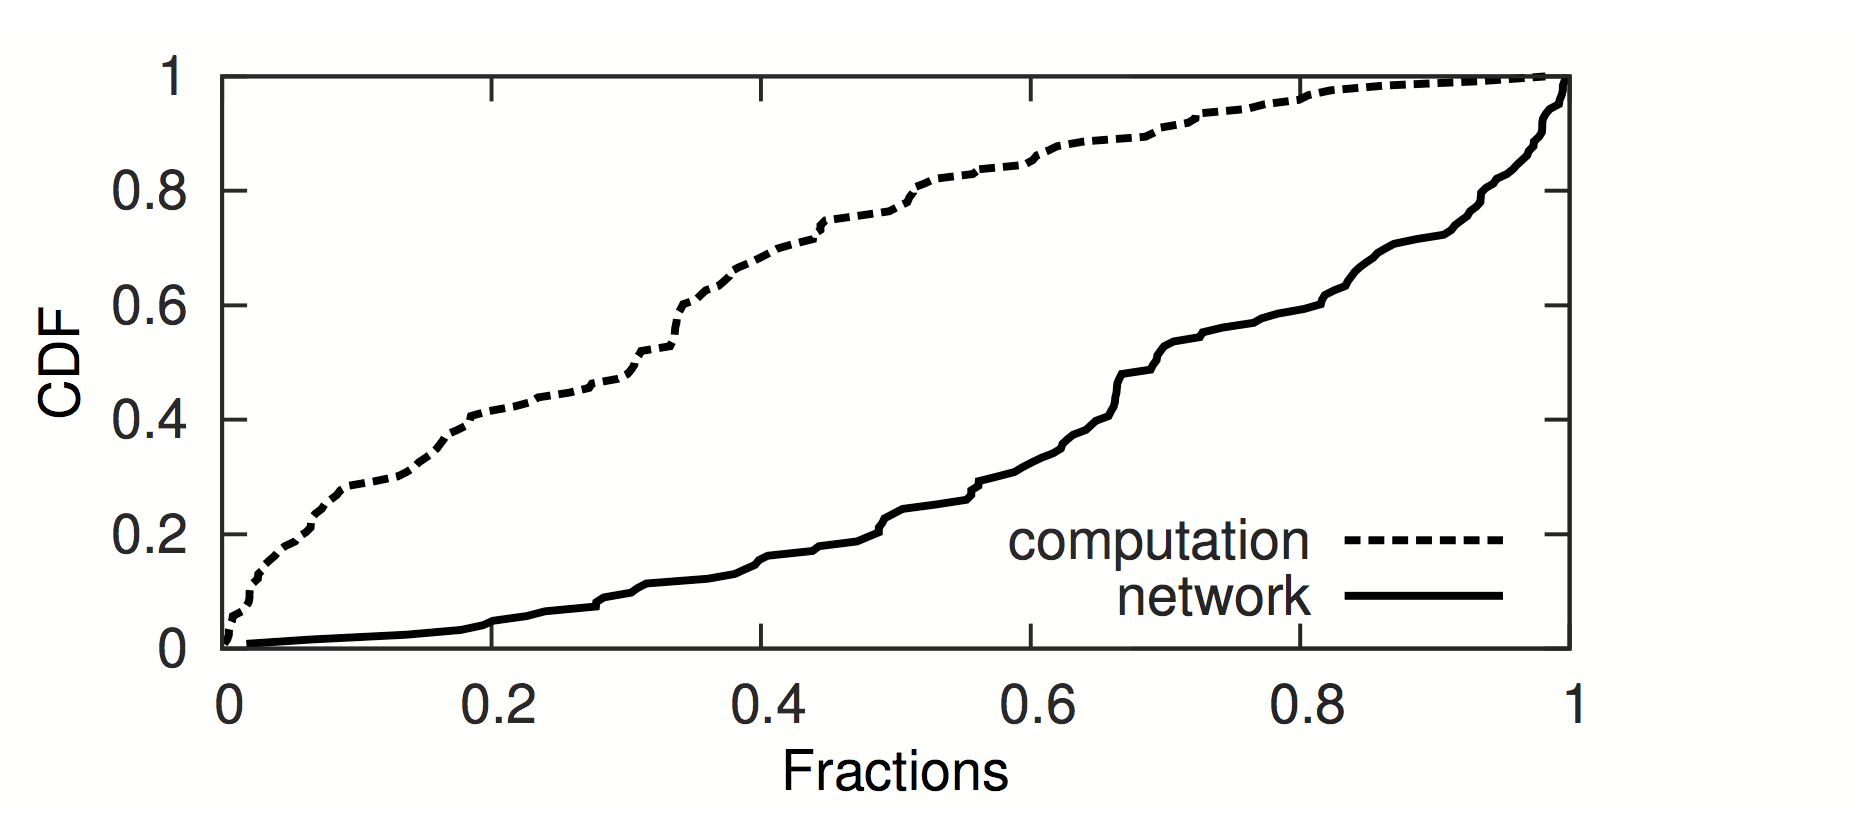
\includegraphics[width=\linewidth]{figs/comp_net_desk.png}
\caption{Runtime information on desktops}
\label{fig:mobile-runtime}
\end{subfigure}
\caption{{\color{red}Figure 1 captioon placeholder}}
\end{figure*}
We propose a new technique to imrpove the page load time by reducing
the javscript time.  In order to do this we are trying to build a new
caching framework for the modern web browsers specifically, Chrome
since it accounts for about 50\% of the market share in terms of
browser usage. Our caching framework will store the javascript
execution result. This can mean a lot of things due to the dynamic
nature javascript. Most of the times it is supposed to be the return
value of the javascript functions. At other times it can be a modified
DOM structure or just some intermediate result which is further
processed by other javascript, later down the execution timeline.  The
expiry of this javascript exectution cache is supposed to be same as
the expire of the javascript source cache.  There are a lot of caveats
to this approach, and in our work we try to essentially explore all of
these.  The biggest challenge with a new caching framework are the
actual modifications to the current browser's code in order to
evaluate the efficacy of our caching frameowork. Since a lot of
browsers already implement caching at the javascript runtime level,
such as compile and parses cache, a lot of this architecure can be
borrowed for the execution cache as well.  Another possible challenge
can be the memory overhead. Most of the popular websites which spend
about 70\% of their time on javascript execution, run about 1000s of
javascript functions. Saving the output of all of these functions can
add an extra overhead on the current browsers. 
